\documentclass{article}
\usepackage{aaai}
\usepackage{graphicx}
\usepackage[toc, page]{appendix}

\title{A Survey of Parallel Search Algorithms}
\author{Seth Lemons \\
Department of Computer Science \\
University of New Hampshire \\
Durham, NH 03824 USA \\
seth.lemons@unh.edu}
\date{\today}

\begin{document}
\maketitle

\begin{abstract}
State space search is an intensive process requiring the examination of many different paths before a solution is found. Any success in doing different parts of a search at the same time can be of great benefit in our increasingly multi-core world. However, states are often interrelated in ways that make parallelization very difficult, causing many proposed algorithms to suffer from synchronization issues or the inability to properly portion out the work. This work attempts to examine the strengths and weaknesses of the most promising parallel search algorithms. We will attempt to determine how well they perform compared to serial algorithms, how scalable they are, and whether they generalize to more than a limited number of domains.
\end{abstract}

\section{Introduction}
Given the large amounts of work that have to be done in state space search, the ability to do more of it at the same time could greatly improve the ability to find fast solutions. With multi-core processors becoming more common and the numbers of cores increasing, doing work in parallel has become much more of a practical consideration. However, designing parallel algorithms is not a trivial activity. Many attempts have been made, and they vary in applicability to given domains, speed in comparison to serial algorithms, optimality of solutions found, and scalability to larger numbers of processor cores. In this study, we evaluate many parallel algorithms on several sets of search problems which can be solved using only system memory. We examine their performance in a setting where all threads share access to main memory.

The algorithms examined are a naive parallel implementation of A*, Parallel Retracting A* \cite{evett:pra}, a parallel version of K Best First Search \cite{felner:kbf}, two versions of Parallel Structured Duplicate Detection \cite{zhou:psd}, and Parallel Best NBlock First \cite{burns:par}. While the details vary, most of the above explore the state space in a best first manner and all are capable of handling problems which can be fit in memory. Only some can handle larger problems which require external memory or limits on total memory use, but we have not tested any in that context.
\section{Algorithms Evaluated}
\subsection{Parallel A*}
The A* algorithm \cite{hart:fbh} is guaranteed to find optimal solutions while searching the least amount of the state space possible with the given heuristic by evaluating the single best node at every step. Because the algorithm requires that the single best node be expanded at each step, it is not possible to directly parallelize the algorithm as it stands. However, our Parallel A* (PA*) algorithm allows threads to select the current best node, ignoring nodes currently being expanded or those created but not yet added to the open list. This means that the first solution returned will not necessarily be optimal and the number of nodes expanded may be greater than serial A*. In addition, threads will have to wait on each other at many points to get nodes off of the open list and insert into the closed list. It is possible that this algorithm, by virtue of doing more than one expansion at a time, could be faster than serial A*. What we will see in our results is that the extra work done and the contention on the open and closed lists exceeds the benefits of parallel execution and makes the algorithm slower than A* for the numbers of threads used.
\subsection{Parallel Retracting A*}
To avoid constant contention on a single open and closed list, Parallel Retracting A* (PRA*) was designed with each thread being given its own lists to search. The determination of which nodes belong to which threads can be done by any hash, although ideally nodes will be hashed in such a way as to split them evenly among the threads. The original design of PRA* was focused on message passing schemes for systems without shared memory, but our implementation uses shared memory to avoid the overhead of messages. In additon, the retracting property of PRA* is a method by which nodes can be condensed back into their parents to allow the algorithm to operate within a memory bound. Because we examined only problems which were known to fit into memory (and because retracting introduces a known deadlock condition), retraction was not built into our implementation. PRA* still finds a suboptimal first solution and may also expand more nodes than A*, but memory contention may be reduced because threads should not always be putting nodes into the same lists at the same time.
\subsection{Parallel KBFS}
One method of reducing contention is to globally synchronize where possible. The K Best First Search algorithm (KBFS) takes the K best nodes from the open list and evaluates them before looking at the open list again. This work can be trivially parallelized by allowing a main thread to pull nodes off the open list and give them to other threads to be expanded. Some contention still occurs when inserting nodes into the open and closed lists, and some threads may spend time waiting on others to finish before the main thread can distribute more work. Like the other algorithms, KBFS can do more work than A* and it still runs the risk of contention in some places. Furthermore, the coordination between the threads can cause inefficiency in various ways. In many cases, the overhead of putting threads to sleep and waking them can add a substantial amount of overhead compared to algorithms in which all threads are constantly attemptimg to do work.
\subsection{Parallel Structured Duplicate Detection}
While PRA* partitions the state space to avoid some contention, the threads must still access each other's data to insert nodes and check for duplicates. The Parallel Structured Duplicate Detection algorithm (PSDD) uses a formal abstraction of the state space to separate nodes into categories and further avoid contention. The abstraction looks much like the original state space but smaller, with all original states mapping to only one abstract state (or nblock) and each nblock having a known set of successors. This successor set is called the duplicate detection scope because exclusive access to this set allows a thread to expand nodes from the original nblock's open list, check the closed list of the successor nblock to which a child node belongs for duplicates, and add the children to the appropriate open lists without obtaining a lock.

This algorithm requires a more in-depth analysis of the state space than a has function, but provides more discreet groupings to which threads can be given exclusive access. The abstraction is maintained as a hash table mapping nblocks to $\sigma$ values representing the number of successors of a given state which are currently in use. When $\sigma$ reaches zero, the nblock and its entire duplicate detection scope are free. A thread which has no nblock to search from takes the lock on the hash table, finds an nblock $b$ with $\sigma$ of zero, and increments the $\sigma$ values of the predeccessors of all nblocks in the duplicate detection scope of $b$. When the thread is done with $b$, the lock is acquired and the $\sigma$ values of the predeccessors of all nblocks in $b$'s duplicate detection scope are decremented. Exclusive access to $b$ and its duplicate detection scope can be guaranteed because for another thread to be able to access $b$ or any nblock in its duplicate detection scope, their sigma values would have to be decremented by the thread currently using them.

The underlying search algorithm originally described proceeds in a breadth first fashion, expanding all nodes from an nblock that belong to the current layer and proceeding to the next layer only after all nodes in the previous layer have been expanded. We implemented one version which uses a standard breadth first search and another which utilizes breadth first heuristic search \cite{zhou:bhs}, called Dynamic PSDD (DynPSDD.) Breadth first heuristic search performs a layer by layer search still, but uses an upper bound on solution cost to prune more expansive nodes off the open list. We acquire this bound by first performing a weighted A* and storing the cost of the solution returned. The time spent on the weighted A* search is factored into all results. While both breadth first search methods guarantee optimal solutions in unit cost worlds, this will not remain true in variable action cost worlds. In addition, outside of a unit cost setting, the number of nodes assigned to a given layer can be very small, causing the time spent switching between nblocks and layers to be much greater.

Much like the hash for PRA*, the size of the abstraction and how evenly the nodes are distributed among the nblocks could affect the amount of overhead required in the search. If nodes are too focused in a small number of nblocks, most of the threads could wait for some time for a few others to finish the current layer before moving on. If nodes are too spread out among too many nblocks, the overhead of switching between nblocks and contention on the hash table for $\sigma$ values could slow performance.
\subsection{Best First Parallel Structured Duplicate Detection}
One adaptation to PSDD suggested by Zhou and Hansen was to search layers in a best first order \cite{zhou:sdd} (BFPSDD) by expanding from the open list of each nblock based on f. The search still expands all nodes in a layer before moving to the next, but the ordering within that layer is different. Because the solution should be one of the lowest cost nodes on its layer, the search can be stopped before fully exploring that layer. Essentially, less work may be performed at the last (and largest) layer if the ordering is good, but nothing is gained at layers without a solution. This modification reduces some of the search cost, but does not resolve the issues with layers in a non-unit cost setting. Another modification was proposed to allow for grouping ranges of f values into a single layer, but that was not included in our implementation. Our implementation of BFPSDD does, however, include the bounding methods used in DynPSDD.
\subsection{Parallel Best Nblock First}
An algorithm that utilizes the abstraction method of PSDD but does not limit itself to one layer at a time is Parallel Best Nblock First (PBNF.) It attempts to utilize a best first order for nblock selection, in addition to a best first ordering of the open lists within nblocks. When a thread has no nblock to search, it acquires the lock on the hash table for the abstraction, finds a list of the nodes with $\sigma$ of zero, and selects from that list the nblock with the lowest f valued node on its open list. Threads expand a minimum number of nodes before attempting to reacquire the lock to get a new nblock with a better f valued node on its open list. If the thread fails to obtain a new nblock (either because the lock was taken by another thread or no better nblock is free), it performs the minimum number of expansions again before repeating its attempt to get a new nblock. The algorithm may find a suboptimal solution first, but it stores incumbent solutions and uses the cost of the current incumbent to prune more expensive nodes off every nblock's open list. When all open lists have emptied, the algorithm terminates and returns the incumbent, which is guaranteed to be the optimal solution if any solution exists.

PBNF avoids the issues of handling layers and, therefore, does not require any modifications to handle variable cost domains or real valued actions. It could also explore a smaller portion of the state space if the ordering is good, but there is always the potential that PBNF could explore further than the deepest layer that PSDD explores, resulting in more total expansions. In addition, PBNF requires an additional parameter that we will see affects the performance of the algorithm non-trivially. Determining the correct value for this parameter for a problem set or domain could be difficult, but it is also possible that this value could be learned online.

The balance between number of nodes per nblock could have an even more stark affect on performance for PBNF than for PSDD, because the number of times threads switch from one nblock to another is not bounded by the depth of the optimal solution. A similar balance is required in the distribution of low f valued nodes between nblocks. If all good nodes are concentrated in a small number of nblocks, most threads will have to expand worse nodes while a few threads do all of the work on the best nodes. Likewise, if good nodes are distributed across too many nblocks, threads will have to switch more often, thus causing more overhead in contention on the hash table.
\subsection{Safe Parallel Best Nblock First}
One issue with PBNF is that nblocks can have good nodes on their open list but be neither free nor actively having nodes expanded from them. A good node could be expanded into an nblock because it is in the duplicate detection scope of $b$ (the active nblock), but $b$ might not immediately be released, so its duplicate detection scope will continue to not be free. Likewise, an nblock could contain nodes that did not previously look promising and thus have other nblocks in its duplicate detection scope be made active. As more of the lower f valued nodes are expanded, the nblock looks better, but still may not become free. Because non-free nblocks are not taken into consideration in the original PBNF specification, both situations could result in extra work being done on less promising nblocks or, in the case of infinite state spaces with sparse solutions, a livelock in which the good nodes are never expanded.

The proposed fix for this issue is to add a flag that can be used to mark nblocks as hot and maintain a $\sigma_h$ value for each nblock, which denotes the number of nblocks in its interference scope (or the nblock's duplicate detection scope and their duplicate detection scopes) which are currently marked as hot. The criteria for an nblock to be considered free, then, are that it have both $\sigma$ and $\sigma_h$ of zero. When a thread evaluates whether it should attempt to switch from $b$ to a new nblock, it examines both the free list and its interference scope. If the best nblock is free, then it simply attempts to get it. However, if the best nblock is in $b$'s interference scope, the thread marks the best nblock $b'$ as hot and increments $\sigma_h$ for all nblocks in $b'$'s interference scope. If $b$ is better than the best free nblock or the best one in $b$'s interference scope, then the thread marks any hot nblock $h$ as no longer hot and decrements $\sigma_h$ for all nblocks in $h$'s interference scope.

The additional effort required to check the interference scope for good nblocks will cause at most a constant factor increase in time because it will be done in all cases where the free list would be checked normally. The greatest cost is most likely to be incurred due to additional nblock switching in attempts to free up promising nblocks. The hope is that the overhead will be balanced out by the more strict adherence to a best first order.
\section{Optimizing Parameters}
Many of the algorithms need only to be given a maximum number of threads to execute. In the case of some algorithms, the number of threads does affect other implicit parameters, such as k in KBFS, the size of the hash function in PRA*, etc. However, several of the algorithms we examined require explicit parameters be defined at the beginning of execution. The values given to these parameters have varying effects on performance, and exploring the results for different values can tell us much about the behavior of the algorithm overall. Results will be shown here for varying parameters on PBNF and BFPSDD because they were the fastest variants and results for other variants (where possible to obtain) were similar in all cases. Other results are shown in the appendix.
\subsection{Abstraction Size}
The number of abstract states used in variants of PSDD and PBNF is a very important parameter, as it determines the number of disjoint duplicate detection scopes and, therefore, the maximum number of threads that can operate in parallel at a given point in time. If we know the number of successors an nblock has, we can easily determine the maximum number of disjoint duplicate detection scopes possible for a given abstraction. It is obvious that we want to have at least as many disjoint duplicate detection scopes as we have threads or we are guaranteed not to have all threads all threads actively searching at any point during execution. We also want fewer abstract states than original states, but this leaves a very large range in between to explore.

In some domains, we have a very fine grained control over the size of the abstraction, allowing us to try many different values and examine their effect on performance. In the grid world domain, for instance, abstracting away the row or column value of a state provides a simple abstraction the size of which is trivial to vary. We implemented such an abstraction by representing all states in the same column (or set of columns) as belonging to a single nblock. We can then vary the number of nblocks in relation to the number of threads (nblocks/thread) and analyze the changes in performance for varying ratios.

\begin{figure}[h!]
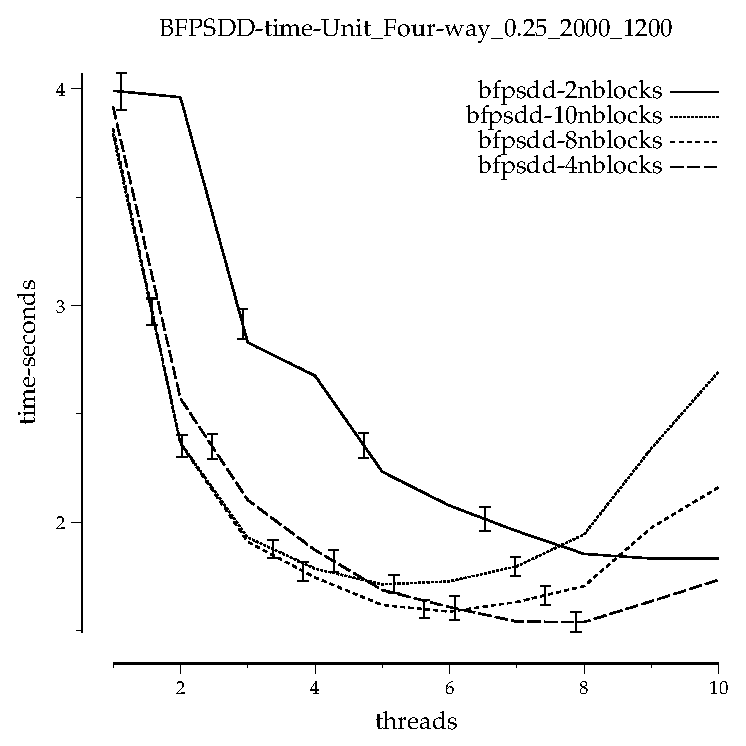
\includegraphics[width=3in]{../graphs/grid_unit_four-way_0.25_2000_1200/BFPSDD-time-Unit_Four-way_0.25_2000_1200.eps}
\caption{Comparison of different nblock/thread ratios on execution time of BFPSDD.}
\label{fig:BFPSDD-nblock-grid}
\end{figure}

\begin{figure}[h!]
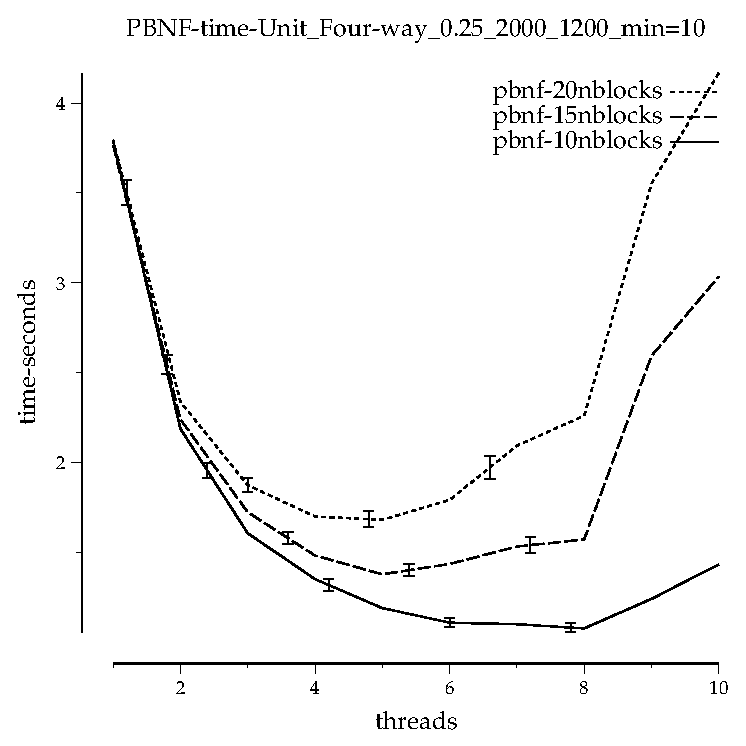
\includegraphics[width=3in]{../graphs/grid_unit_four-way_0.25_2000_1200/PBNF-time-Unit_Four-way_0.25_2000_1200_min=10.eps}
\caption{Comparison of different nblock/thread ratios on execution time of PBNF in unit cost grid world.}
\label{fig:PBNF-nblock-grid}
\end{figure}

As we can see from Figure \ref{fig:BFPSDD-nblock-grid} and Figure \ref{fig:PBNF-nblock-grid}, not only do both PBNF and BFPSDD start to perform worse as the number of nblocks per thread increases beyond a value of 10, but the shape of the curve actually changes. Having too many nblocks does not simply slow these algorithms down, it makes them perform worse as the number of threads increases. Values below 10 are not shown because they caused the algorithms to take too long to measure over a large enough problem set. The same results are true, although with variation in the optimal ratio, for other variants of these algorithms, as shown in Figure \ref{fig:nblock-grid} in the appendix. Determining the appropriate ratio before execution, however, is a non-trivial problem.

\begin{figure}[h!]
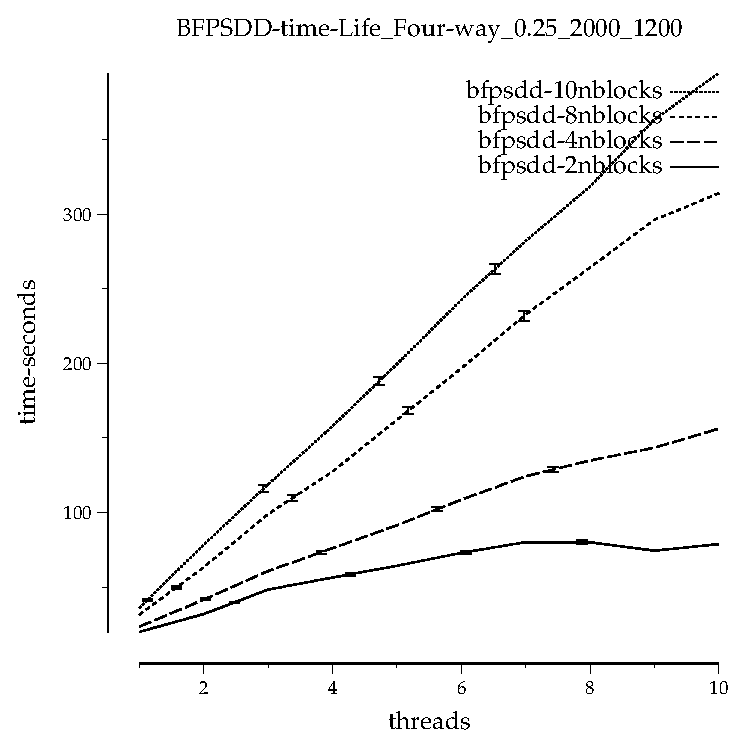
\includegraphics[width=3in]{../graphs/grid_life_four-way_0.25_2000_1200/BFPSDD-time-Life_Four-way_0.25_2000_1200.eps}
\caption{Comparison of different nblock/thread ratios on execution time of BFPSDD in life cost grid world.}
\label{fig:BFPSDD-nblock-life}
\end{figure}

\begin{figure}[h!]
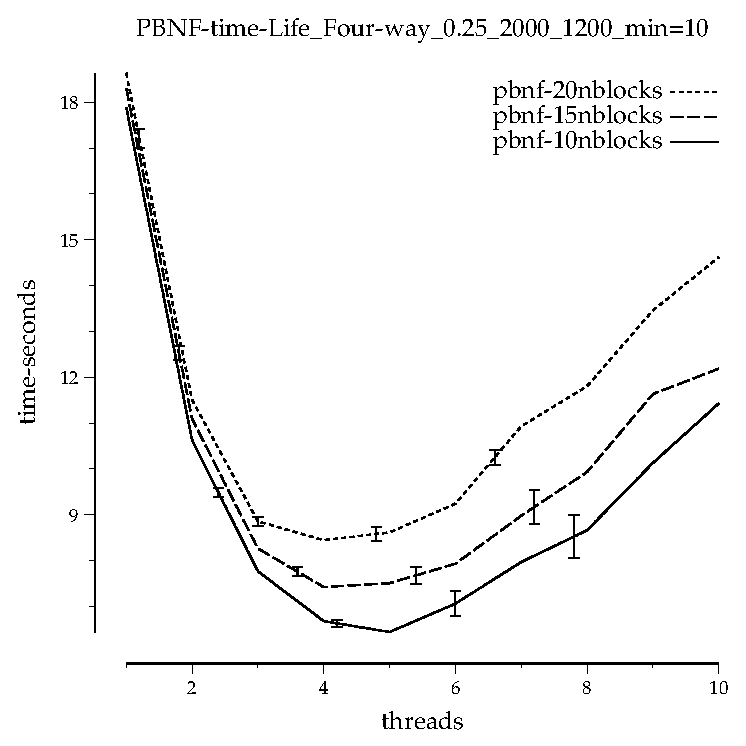
\includegraphics[width=3in]{../graphs/grid_life_four-way_0.25_2000_1200/PBNF-time-Life_Four-way_0.25_2000_1200_min=10.eps}
\caption{Comparison of different nblock/thread ratios on execution time of PBNF in life cost grid world.}
\label{fig:PBNF-nblock-life}
\end{figure}

Both BFPSDD and PBNF have a clearly discernable best ratio of nblocks to threads in life cost grid world problems tested, although their behavior overall is less desirable. Figure \ref{fig:BFPSDD-nblock-life} and Figure  \ref{fig:PBNF-nblock-life} show that the ratios of 2 and 10 are best for PSDD and PBNF respectively in the life cost instances they were run on. No data is reported for other variants of PSDD or ratios less than 10 for PBNF because all of them were too slow to be tested in a reasonable amount of time.

In other domains or when a different abstraction is used, control over the abstraction size is more coarse. The abstraction most commonly used in the sliding tile puzzle is to ignore the locations of all but some subset of the tiles. Adding or removing a tile from the set we pay attention to, however, changes the number of abstract states dramatically. Likewise, we can partition the grid world board into an abstract grid where each abstract grid location contains a set of neighboring original grid locations. Again, the number of abstract states increases or decreases dramatically when we increase the factor by which we divide the board. Results for a domain should still apply in regard to the correct abstraction size, however, even if we cannot control the ratio as precisely.
\subsection{Weight for Preliminary Search}
The weight used in the preliminary search for DynPSDD and BFPSDD affects the optimality of the solution found and, therefore, the amount of pruning that can be done during the search. For higher weights, the initial search should be faster, but little pruning can be done. When weights approach 1, though, the initial search will take longer with no benefit from parallelization and much of the work done in the actual PSDD search will be reproducing work done by the weighted search.

\begin{figure}[h!]
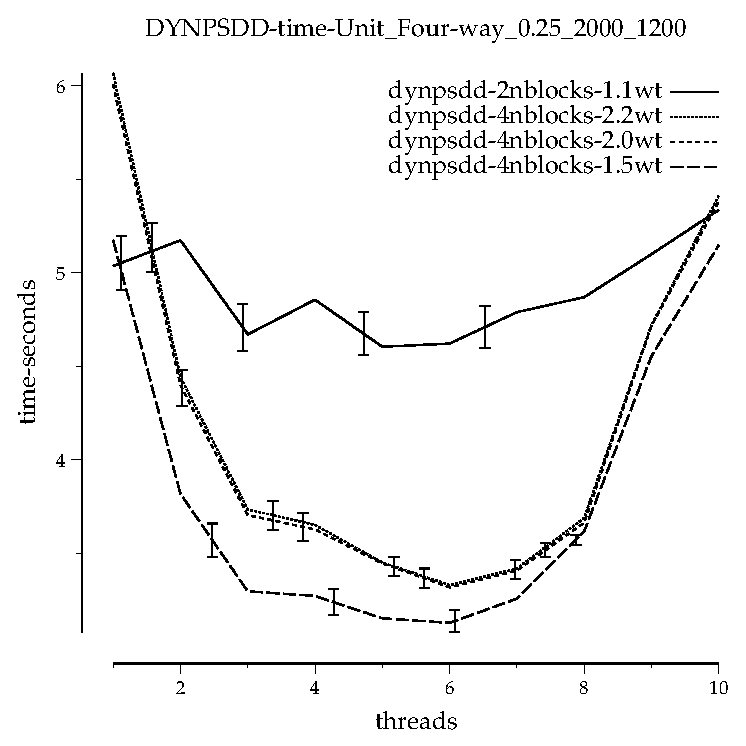
\includegraphics[width=3in]{../graphs/grid_unit_four-way_0.25_2000_1200/DYNPSDD-time-Unit_Four-way_0.25_2000_1200.eps}
\caption{Comparison of weights for the preliminary weighted A* search and their effect on overall search time.}
\label{fig:DynPSDD-weight-grid}
\end{figure}

As Figure \ref{fig:DynPSDD-weight-grid} shows, the weight used can greatly affect the cost of the overall search. With very low weights, time is always high and there is only minor variation because of the number of threads used for the actual PSDD search. The weight of 1.5 worked best in our grid world tests, finding an adequate solution relatively fast, allowing PSDD to do less work without waiting as long to begin. Higher weights not only run the risk of returning poorer solutions which negatively affect pruning, but in some cases they can also cause the weighted A* search to run longer than at lower weights because it veers too far of on bad paths.

Additionally, there appears to be a relationship between the weight of the initial search and the best number of nblocks per thread. For a weight of 1.1, the search performs best on average with 2 nblocks per thread, while for all other weights the best performance is at 4 nblocks per thread. Results for various weights in relation to the nblock to thread ratio can be seen in Figure \ref{fig:weight-grid} of the appendix. It is quite possible that with a near-optimal bound on solution cost, the algorithm performs better with a smaller abstraction because there are fewer nodes to spread around.
\subsection{Minimum Expansions}
One variable unique to PBNF variants is the number of expansions to perform before attempting to find a new nblock to work on. In the ideal situation, this parameter would keep threads from contending over the hash table of $\sigma$ values, but it could also cause them to expand far more nodes than necessary. The best value for this will change based not only the problem at hand, but the abstraction size and how well good states are distributed among nblocks.

\begin{figure}[h!]
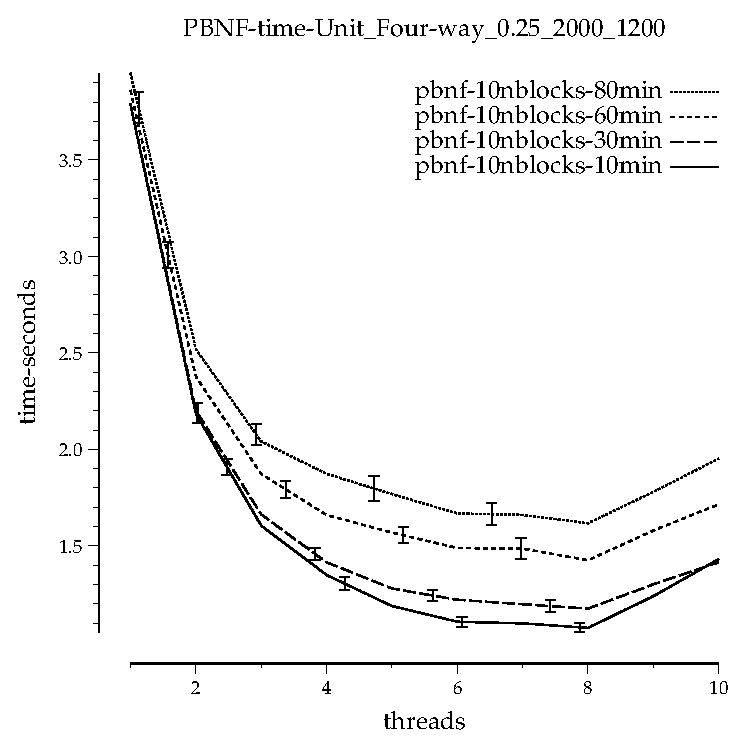
\includegraphics[width=3in]{../graphs/grid_unit_four-way_0.25_2000_1200/PBNF-time-Unit_Four-way_0.25_2000_1200.eps}
\caption{Different values for minimum expansions in PBNF on unit cost grids.}
\label{fig:PBNF-min-grid}
\end{figure}

\begin{figure}[h!]
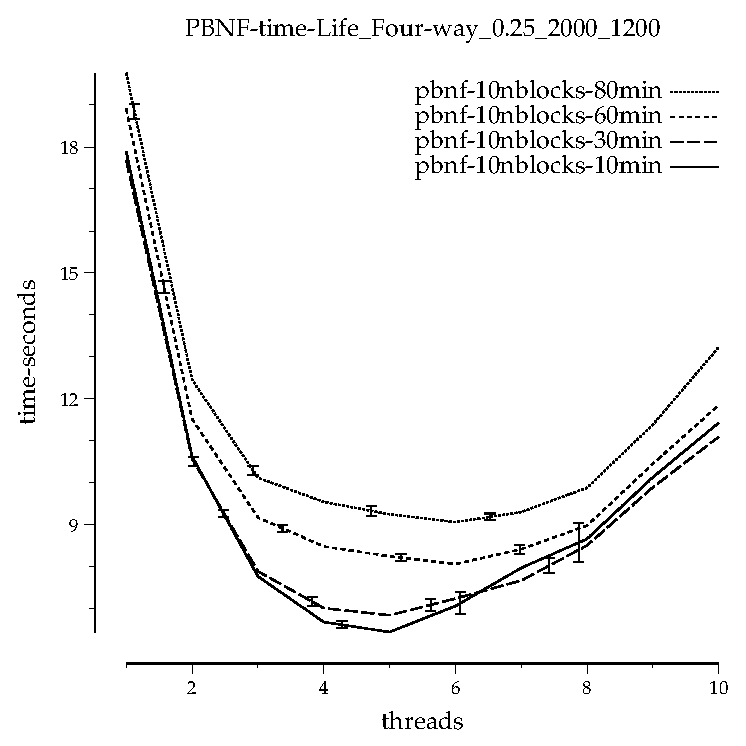
\includegraphics[width=3in]{../graphs/grid_life_four-way_0.25_2000_1200/PBNF-time-Life_Four-way_0.25_2000_1200.eps}
\caption{Different values for minimum expansions in PBNF on life cost grids.}
\label{fig:PBNF-min-life}
\end{figure}

In our grid world tests, 10 minimum expansions before switching seems to lead to the best performance. Figure \ref{fig:PBNF-min-grid} illustrates that values above 10 increase performance times, shifting the line upward without substantially changing its shape. Higher values do not appear to make the algorithm less scalable, however. Values below 10 caused such bad performance that we were again unable to complete tests on them. The distinction is less clear in the life cost tests shown in Figure \ref{fig:PBNF-min-life}, indicating that variable edge costs may necessitate a more flexible method of determining this value.

\begin{figure}[h!]
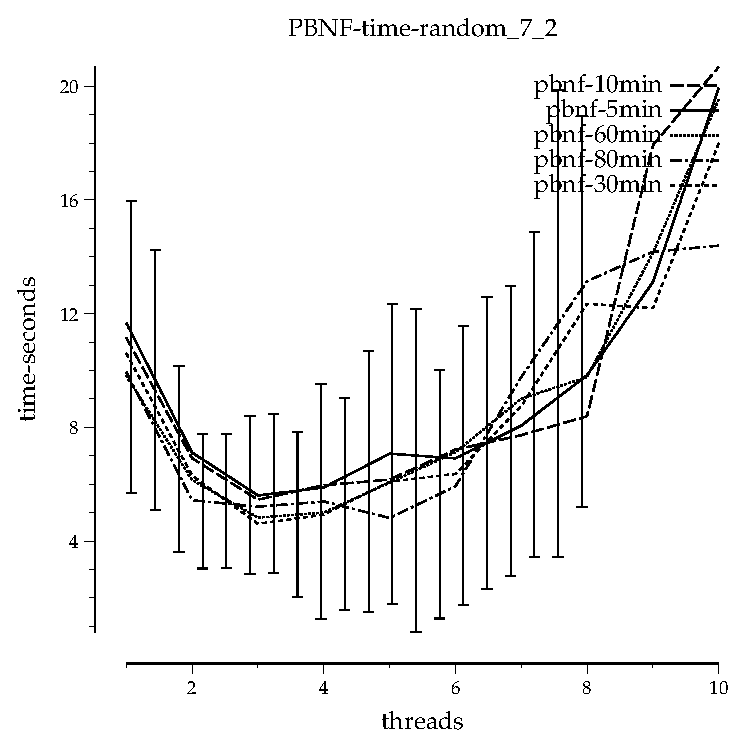
\includegraphics[width=3in]{../graphs/tiles_random_7_2/PBNF-time-random_7_2.eps}
\caption{Different values for minimum expansions in PBNF on 7x2 sliding tile puzzles.}
\label{fig:PBNF-min-tile}
\end{figure}

Optimizing the minimum number of expansions proved much more complicated for sliding tile puzzles. While 30 minimum expansions gives the best average performance, results varied widely enough that no option is clearly the best. Figure \ref{fig:PBNF-min-tile} shows that the confidence intervals of almost all minimum expansion values overlap, even though the instances used did not vary greatly in difficulty. It is possible that either the abstraction does not suit all problems equally well or that there are other factors of sliding tile puzzles which affect the algorithm in ways we have yet to understand.
\section{Comparison}
Having determined the best parameters to use with each algorithm for the domains we tested them on, the next step is to compare their performance across those domains. We show results for unit cost grid world, life cost grid world, and the 7x2 sliding tile puzzle for all algorithms which performed well enough to complete execution on the given domain. All parameters were set to the best known value to compare best case performance. We test with 1 to 8 threads because the machine we tested on has 8 cores.

\begin{figure}[h!]
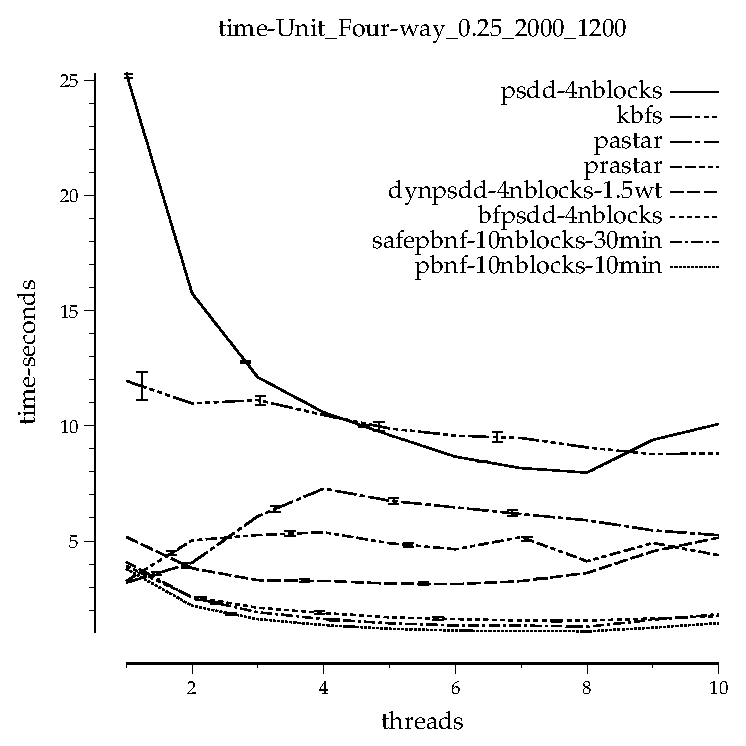
\includegraphics[width=3in]{../graphs/seth/time-Unit_Four-way_0.25_2000_1200.eps}
\caption{Comparison of all algorithms on unit cost grid world problems.}
\label{fig:comp-grid}
\end{figure}

Figure \ref{fig:comp-grid} shows all algorithms on unit cost grid world instances. It is interesting to note that with a single thread, PA* and PRA* are equivalent to serial A*. Their execution time increases steeply at first and gradually decreases as threads are added. PRA* seems to have more erratic behavior than PA*, most likely because the way threads are hashed changes based on the number of threads and the interactions between threads are slightly more complex. While BFPSDD, PBNF, and SafePBNF start out slightly more expensive than serial A*, their runtimes slowly decrease and are consistently the best. KBFS is a real oddity because, in theory, its performance at 1 thread should also be roughly equivalent to A*. However, it appears that the overhead of synchronizing the main thread and the search thread(s) is quite large. It seems to benefit from more threads, but is still far worse off than most of the other algorithms at any point tested. We can see that SafePBNF is slightly slower than PBNF, most likely due to additional overhead of checking the protection scope. BFPSDD is slower than both variants of PBNF, probably because of the fact that it expands all nodes at every layer but the last. Dynamic PSDD comes close to being in the set of good algorithms at times, but also seems to increase in execution time for higher numbers of threads. The cause of this slowing down is not immediately apparent, especially considering the fact that both other variants of PSDD do not suffer from it. PSDD behaves quite poorly because it is searching far more nodes than any other algorithm, and the cost is only later outweighed by the benefits of parallel execution at higher numbers of threads.

\begin{figure}[h!]
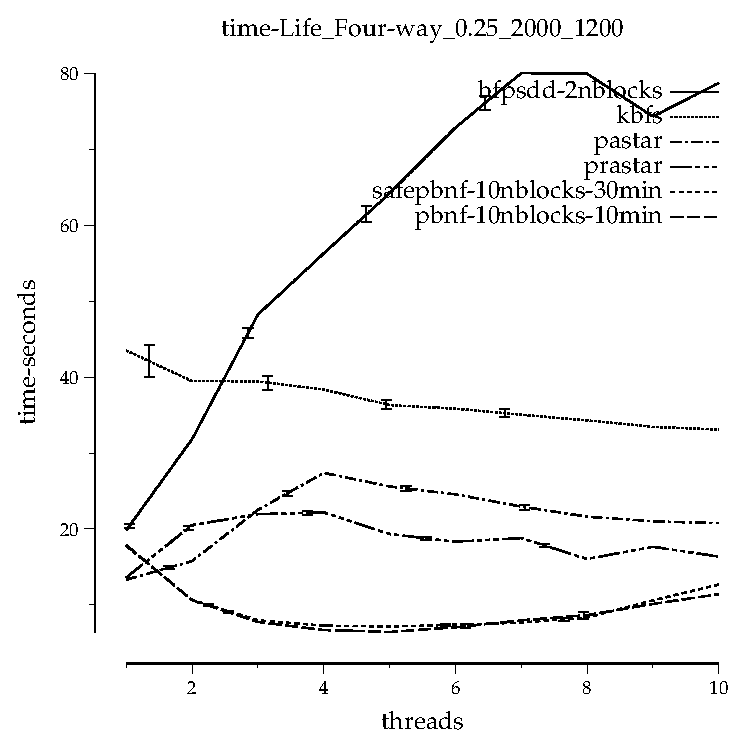
\includegraphics[width=3in]{../graphs/seth/time-Life_Four-way_0.25_2000_1200.eps}
\caption{Comparison of all algorithms on life cost grid world problems.}
\label{fig:comp-life}
\end{figure}

The comparison of most of the algorithms, shown in Figure \ref{fig:comp-life}, illustrates that non-unit action cost has a dramatic effect on many of them. The behavioe exhibited by PA* and PRA* is essentially the same as unit cost, increasing for the first few threads and gradually decreasing. KBFS also performs roughly the same as before, still being overwhelmed by synchronization costs. BFPSDD behaves quite strangely, with execution times increasing steadily for each thread added. This behavior is because of the layered nature of PSDD algorithms and the fact that to return an optimal solution, g costs, rather than depth of a node, have to be used to determine layers. With multiple layers at each depth level, more time is spent switching between nblocks with very small open lists. The other PSDD variants behaved even more poorly than BFPSDD, as is to be expected. The PBNF variants perform relatively well, outperforming the other algorithms at almost all points past 1 thread. The disappointing fact is that both PBNF and SafePBNF require longer execution times for more threads after a certain point. This may be due to the abstraction becoming too large at higher numbers of threads because we maintain a ratio of nblocks to threads, rather than a constant number of nblocks. As we have said, too many nblocks could increase overhead from switching when nblocks empty too easily.

\begin{figure}[h!]
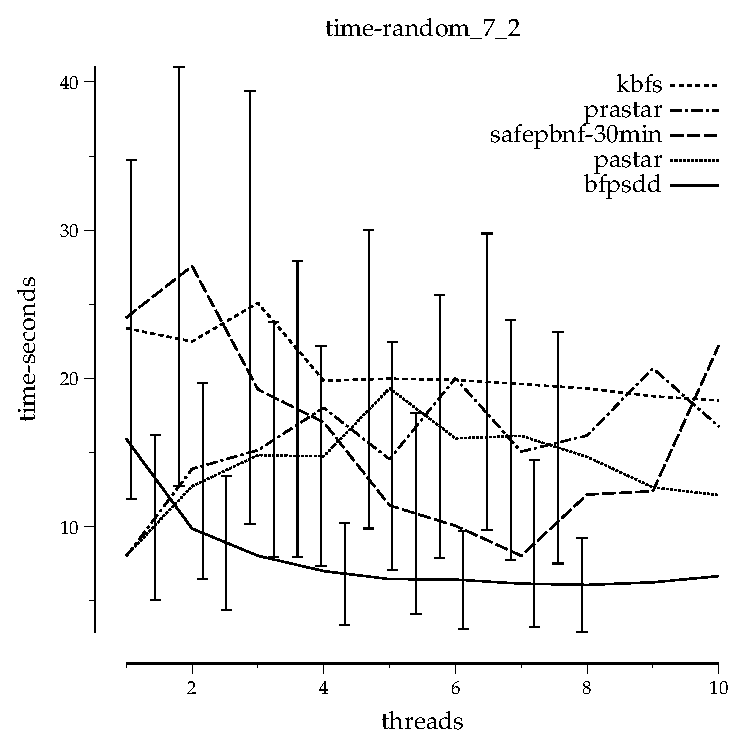
\includegraphics[width=3in]{../graphs/seth/time-random_7_2.eps}
\caption{Comparison of all algorithms on 7x2 sliding tile puzzles.}
\label{fig:comp-tile}
\end{figure}

Finally, the results of testing on 7x2 sliding tile puzzles are shown in Figure \ref{fig:comp-tile}. As the large confidence intervals indicate, behavior for all algorithms was erratic, possibly due to variance in difficulty of the instances used. Execution times of PA* and PRA* increase at the start, just as before, but their slope after that point is not clear. As always, KBFS starts off very poorly and slowly improves its time, albeit with a strange jump upward and back down between 2 and 4 threads. The abstraction used for the PSDD and PBNF variants was quite small, causing even further anomalies in some of their results. SafePBNF starts out almost as poorly as KBFS, improves, and then seems to become worse again. PBNF begins, as usual, very near serial A*, improving as it goes, but it starts to do worse for higher numbers of threads. BFPSDD seems to be the only algorithm to truly behave well in this example. It starts out somewhat worse than serial A*, but consistently decreases execution times as threads are added. Its good performance in sliding tiles makes sense in light of the fact that it was originally tested by Zhou and Hansen in this domain. Also, its method of searching fits for a domain in which the actions are unit cost and the heuristic is admissible but not extremely accurate.
\section{Future Work}
One obvious limitation of the evaluations done here is the number of threads used. In several cases, algorithms are improving in speed, but we cannot be sure that they would continue doing so. It is very difficult to make definite statements about scalability without further information.
While attention was paid to the size of the abstraction used for PSDD and PBNF variants, examination of the properties that make an abstraction useful to such algorithms and how big of an effect these properties have on execution time could be very informative. In addition, PRA* could be tested with has functions of varying quality. Both abstractions and hashes could be tested to see how well they split up the state space and how evenly they distribute good nodes.
The problem instances used for our tests were the same size and did not vary much in difficulty. Future evaluations of these algorithms could look at how difficult it is to optimize parameters over larger distributions of problem size and difficulty. If good parameters cannot be found in such a situation, it would make a much stronger case for automatically learning or adjusting these values for each problem solved.
Several changes could be made to the algorithms' implementations to test whether the problems observed could be circumvented. Because PRA* was originally designed for message passing systems, the effect of contention on the algorithm could be different if message passing were simulated in a threaded system, rather than allowing threads to contend over each other's open lists. Likewise, it could be instructive to implement the modification to PSDD variants by which layers could represent a range of values, rather than a single value. This could improve their performance in the life cost problems.
\section{Acknowledgements}
My thanks to Ethan Burns, Wheeler Ruml, and Rong Zhou for collaboration on implementation and testing of these algorithms.

\bibliography{master}
\bibliographystyle{aaai}

\begin{appendices}
\begin{figure*}[h!]
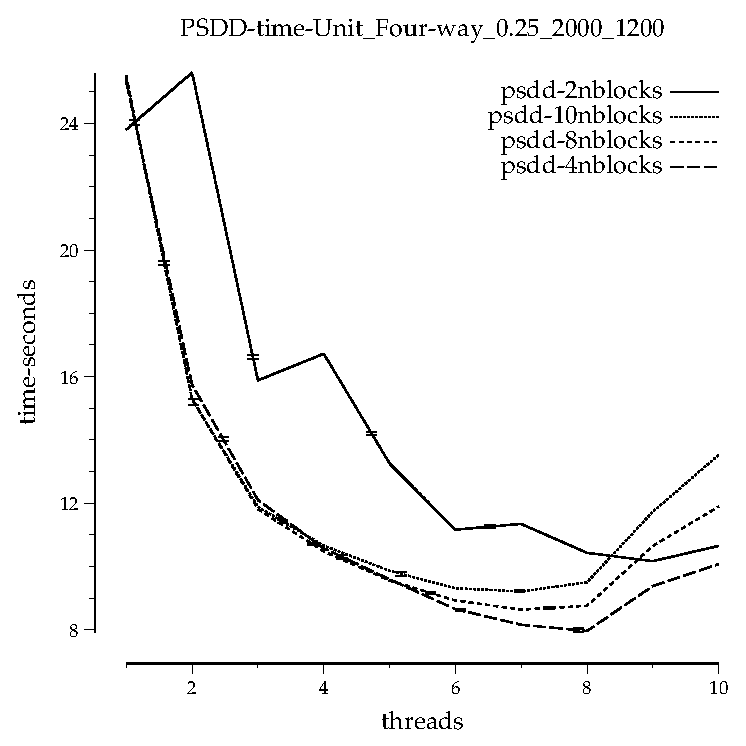
\includegraphics[width=3in]{../graphs/grid_unit_four-way_0.25_2000_1200/PSDD-time-Unit_Four-way_0.25_2000_1200.eps}
\includegraphics[width=3in]{../graphs/grid_unit_four-way_0.25_2000_1200/DYNPSDD-time-Unit_Four-way_0.25_2000_1200_weight=1.5.eps}
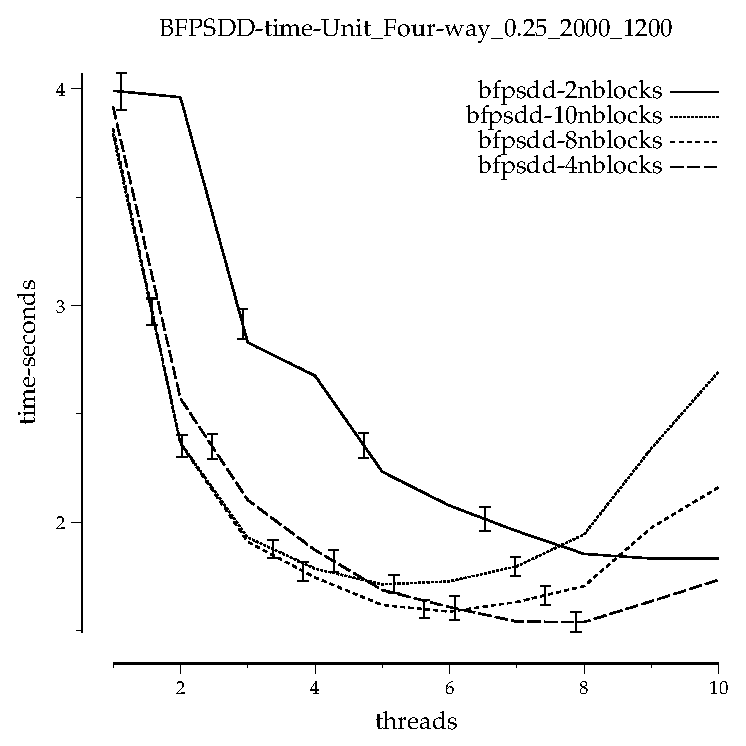
\includegraphics[width=3in]{../graphs/grid_unit_four-way_0.25_2000_1200/BFPSDD-time-Unit_Four-way_0.25_2000_1200.eps}
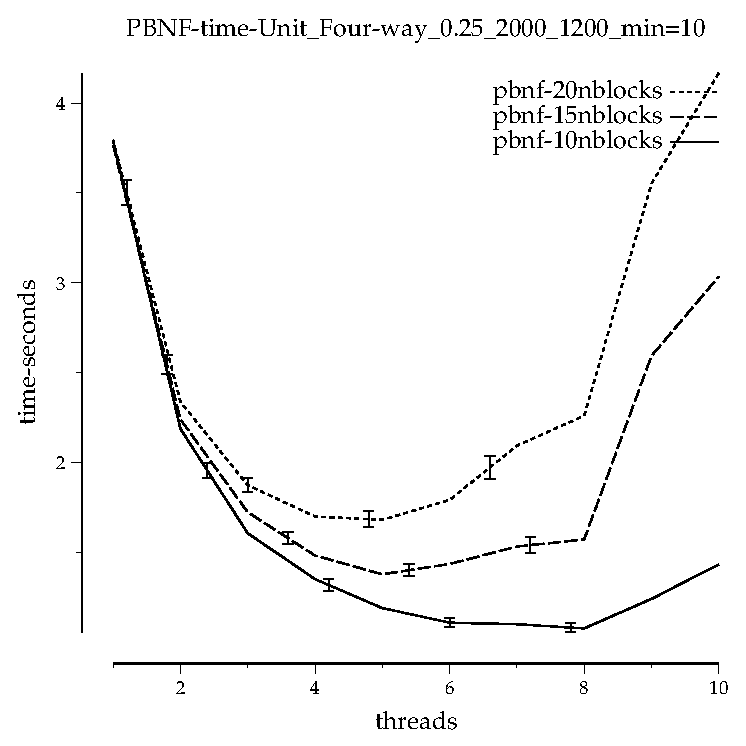
\includegraphics[width=3in]{../graphs/grid_unit_four-way_0.25_2000_1200/PBNF-time-Unit_Four-way_0.25_2000_1200_min=10.eps}
\caption{Comparison of different nblock/thread ratios on execution time of PSDD, DynPSDD, BFPSDD, PBNF, and Safe PBNF.}
\label{fig:nblock-grid}
\end{figure*}

\begin{figure*}[h!]
\begin{center}
\includegraphics[width=3in]{../graphs/grid_unit_four-way_0.25_2000_1200/DYNPSDD-time-Unit_Four-way_0.25_2000_1200_weight=1.1.eps}
\includegraphics[width=3in]{../graphs/grid_unit_four-way_0.25_2000_1200/DYNPSDD-time-Unit_Four-way_0.25_2000_1200_weight=1.5.eps}
\includegraphics[width=3in]{../graphs/grid_unit_four-way_0.25_2000_1200/DYNPSDD-time-Unit_Four-way_0.25_2000_1200_weight=2.0.eps}
\includegraphics[width=3in]{../graphs/grid_unit_four-way_0.25_2000_1200/DYNPSDD-time-Unit_Four-way_0.25_2000_1200_weight=2.2.eps}
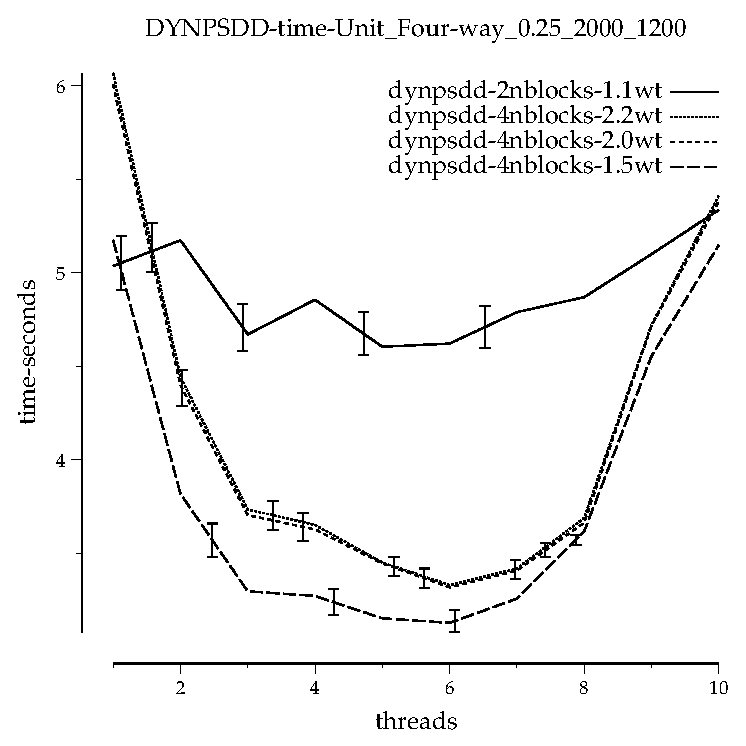
\includegraphics[width=3in]{../graphs/grid_unit_four-way_0.25_2000_1200/DYNPSDD-time-Unit_Four-way_0.25_2000_1200.eps}
\caption{DynPSDD on unit cost grid world boards.}
\label{fig:DynPSDD-grid}
\end{center}
\end{figure*}

\begin{figure*}[h!]
\includegraphics[width=3in]{../graphs/grid_unit_four-way_0.25_2000_1200/DYNPSDD-time-Unit_Four-way_0.25_2000_1200_weight=1.1.eps}
\includegraphics[width=3in]{../graphs/grid_unit_four-way_0.25_2000_1200/DYNPSDD-time-Unit_Four-way_0.25_2000_1200_weight=1.5.eps}
\includegraphics[width=3in]{../graphs/grid_unit_four-way_0.25_2000_1200/DYNPSDD-time-Unit_Four-way_0.25_2000_1200_weight=2.0.eps}
\includegraphics[width=3in]{../graphs/grid_unit_four-way_0.25_2000_1200/DYNPSDD-time-Unit_Four-way_0.25_2000_1200_weight=2.2.eps}
\caption{Different weights with different nblock ratios in DynPSDD.}
\label{fig:weight-grid}
\end{figure*}

\begin{figure*}[h!]
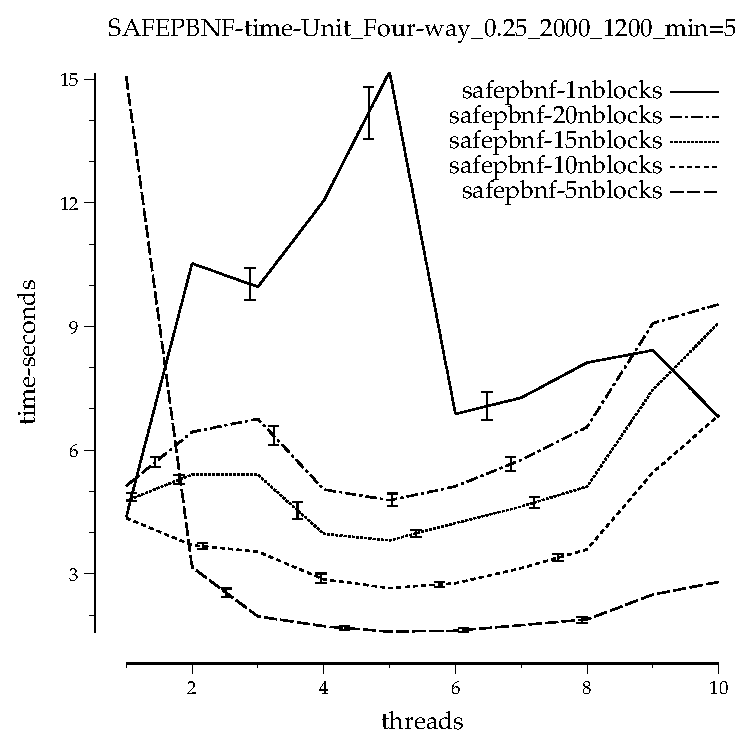
\includegraphics[width=3in]{../graphs/grid_unit_four-way_0.25_2000_1200/SAFEPBNF-time-Unit_Four-way_0.25_2000_1200_min=5.eps}
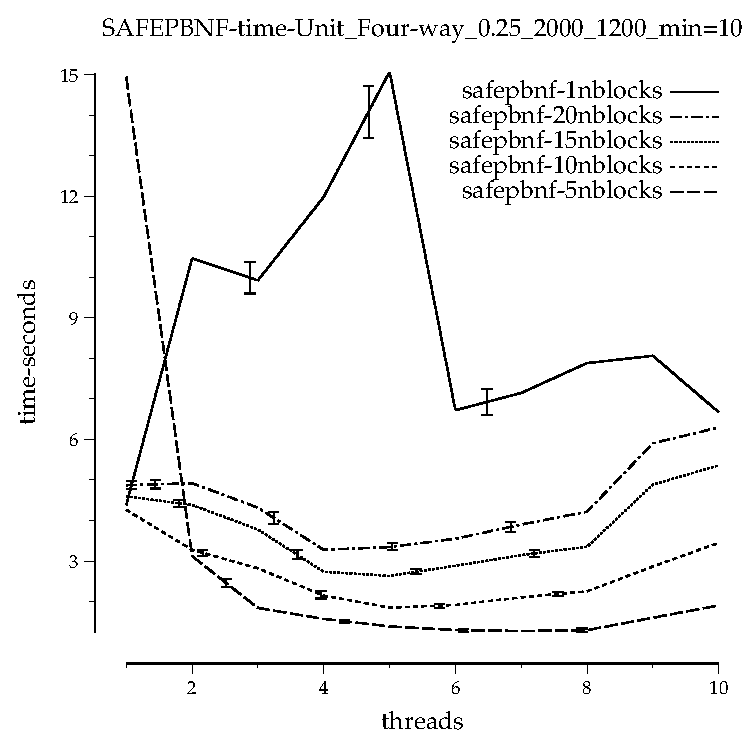
\includegraphics[width=3in]{../graphs/grid_unit_four-way_0.25_2000_1200/SAFEPBNF-time-Unit_Four-way_0.25_2000_1200_min=10.eps}
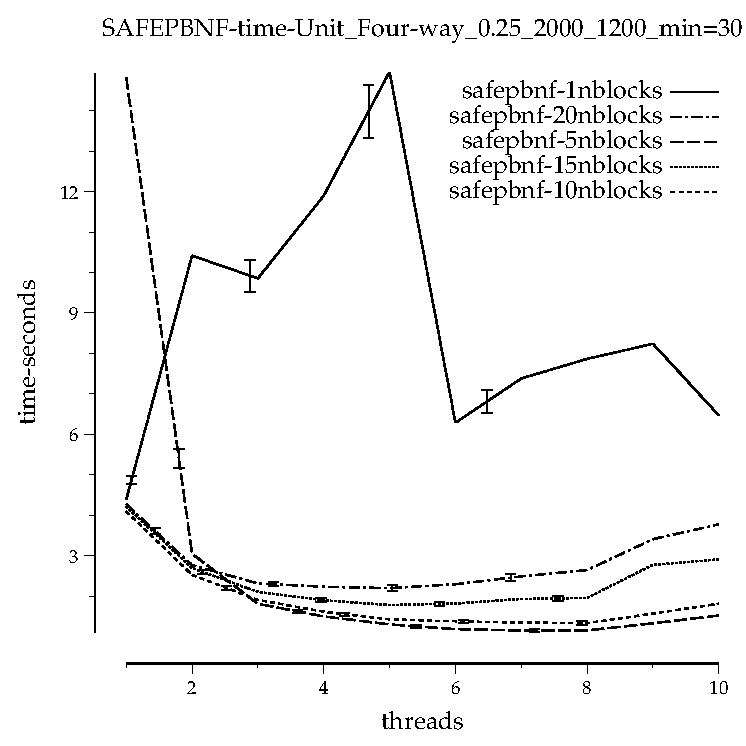
\includegraphics[width=3in]{../graphs/grid_unit_four-way_0.25_2000_1200/SAFEPBNF-time-Unit_Four-way_0.25_2000_1200_min=30.eps}
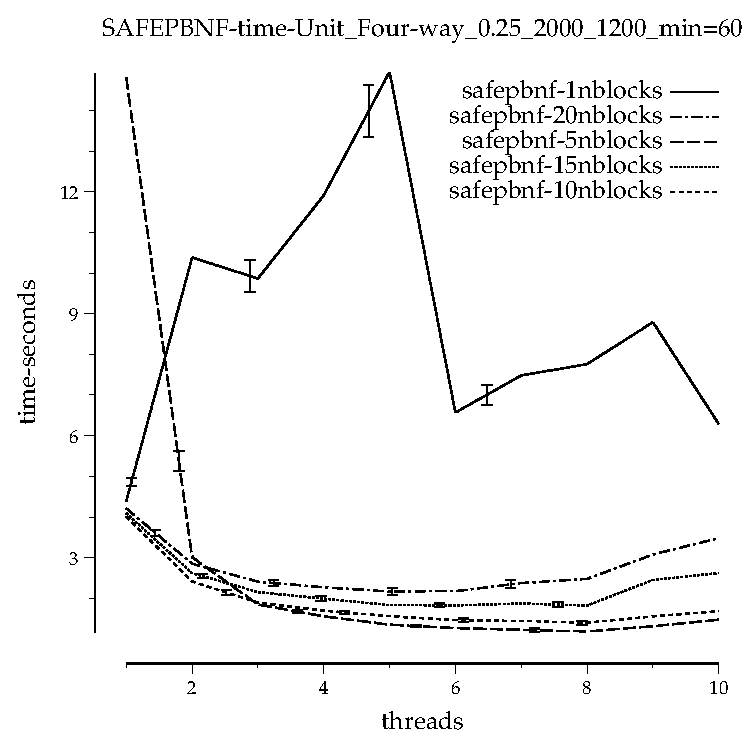
\includegraphics[width=3in]{../graphs/grid_unit_four-way_0.25_2000_1200/SAFEPBNF-time-Unit_Four-way_0.25_2000_1200_min=60.eps}
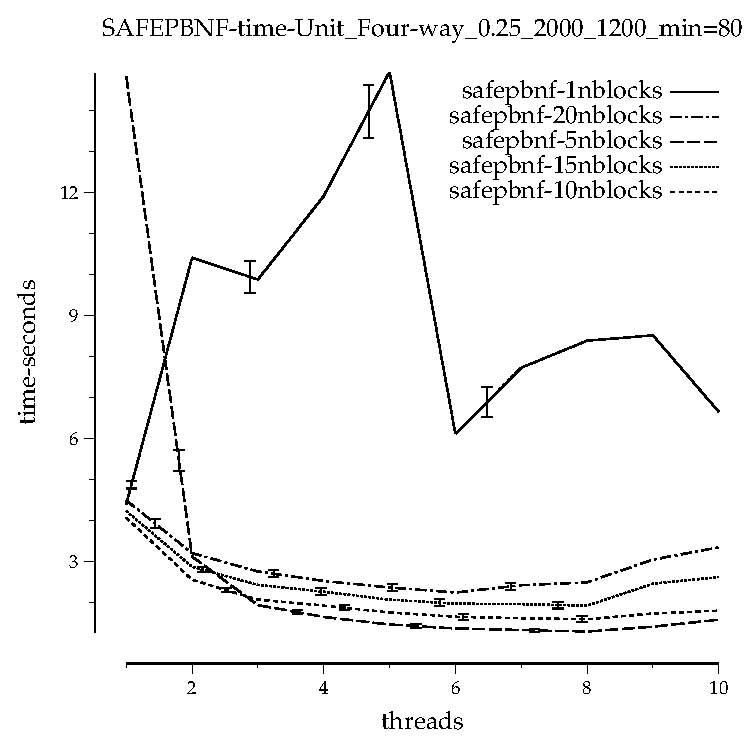
\includegraphics[width=3in]{../graphs/grid_unit_four-way_0.25_2000_1200/SAFEPBNF-time-Unit_Four-way_0.25_2000_1200_min=80.eps}
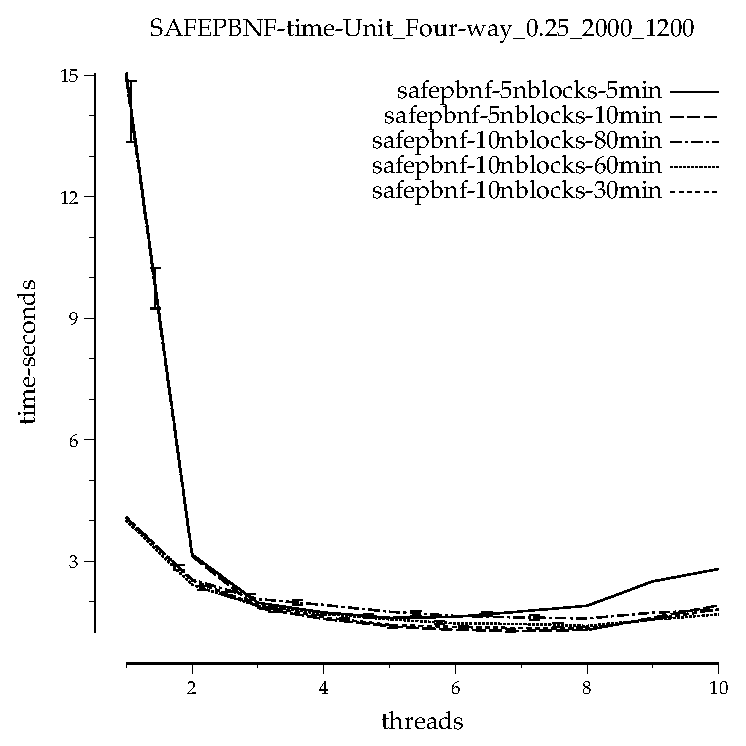
\includegraphics[width=3in]{../graphs/grid_unit_four-way_0.25_2000_1200/SAFEPBNF-time-Unit_Four-way_0.25_2000_1200.eps}
\caption{Safe PBNF on unit cost grid world boards.}
\label{fig:SafePBNF-grid}
\end{figure*}

\begin{figure*}[h!]
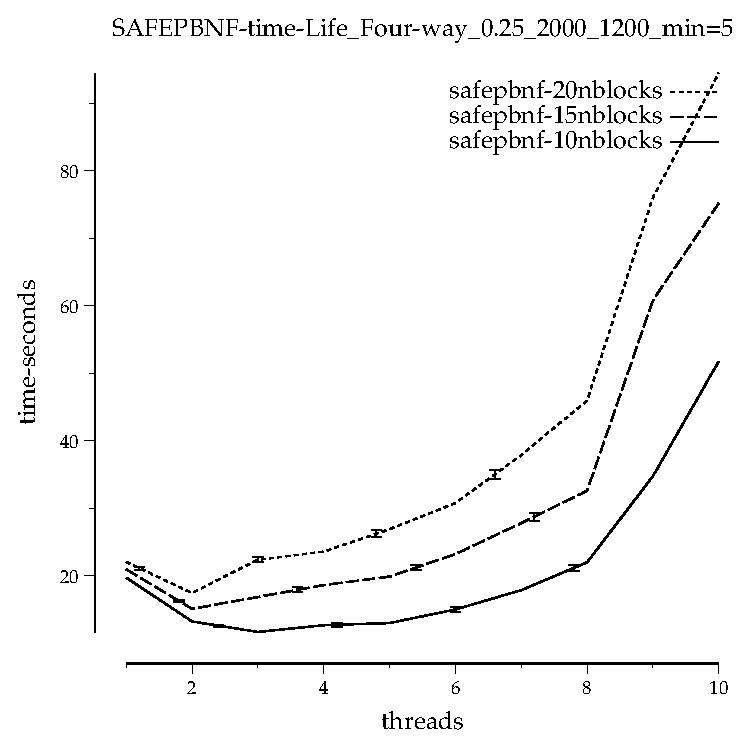
\includegraphics[width=3in]{../graphs/grid_life_four-way_0.25_2000_1200/SAFEPBNF-time-Life_Four-way_0.25_2000_1200_min=5.eps}
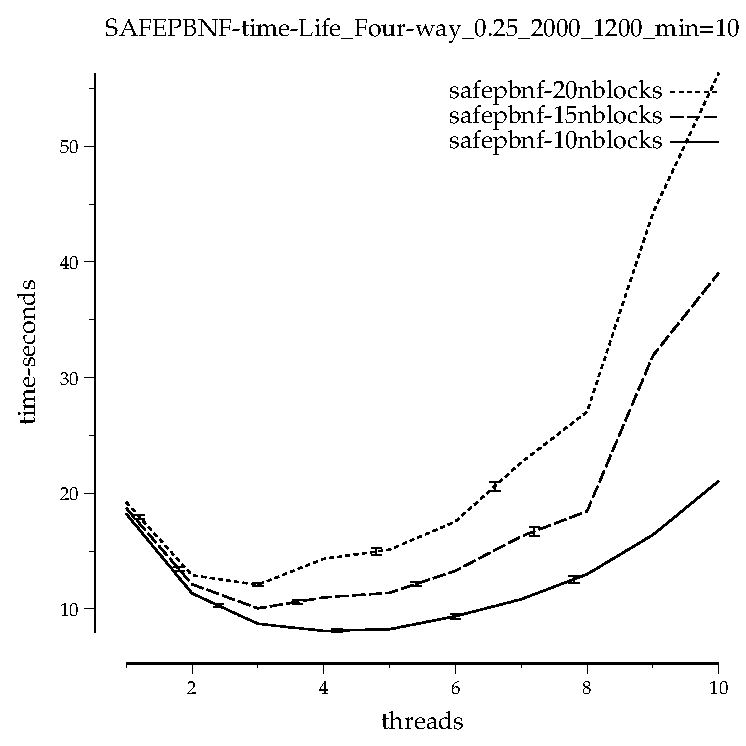
\includegraphics[width=3in]{../graphs/grid_life_four-way_0.25_2000_1200/SAFEPBNF-time-Life_Four-way_0.25_2000_1200_min=10.eps}
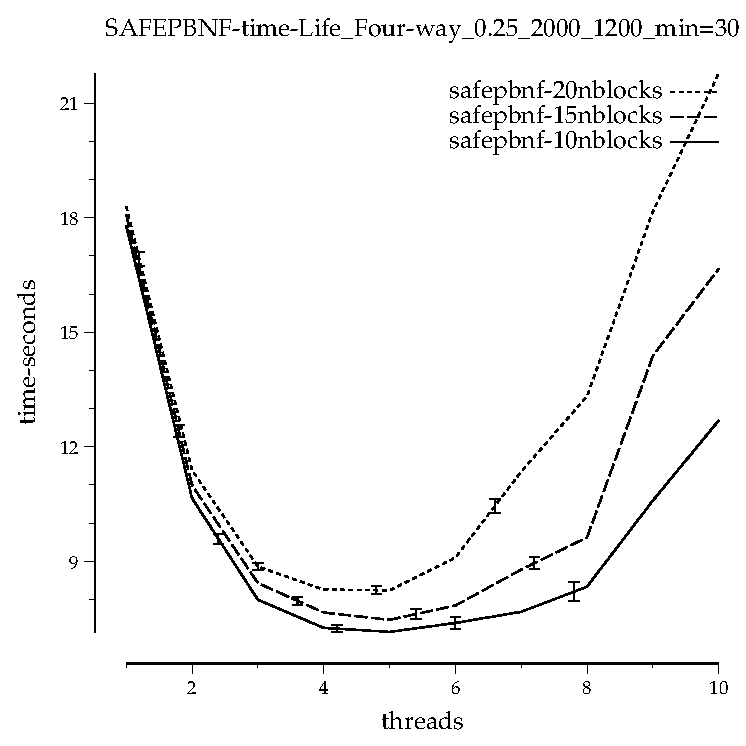
\includegraphics[width=3in]{../graphs/grid_life_four-way_0.25_2000_1200/SAFEPBNF-time-Life_Four-way_0.25_2000_1200_min=30.eps}
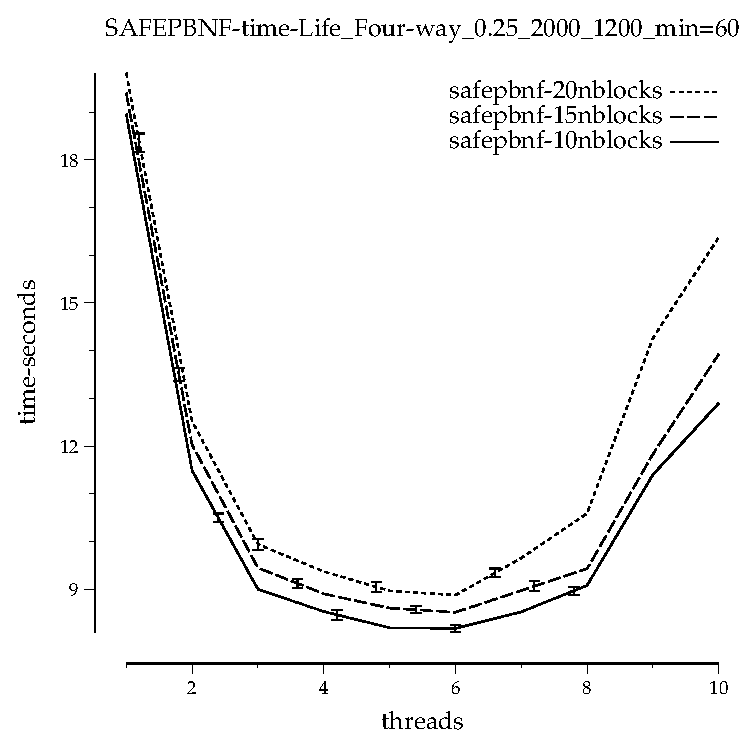
\includegraphics[width=3in]{../graphs/grid_life_four-way_0.25_2000_1200/SAFEPBNF-time-Life_Four-way_0.25_2000_1200_min=60.eps}
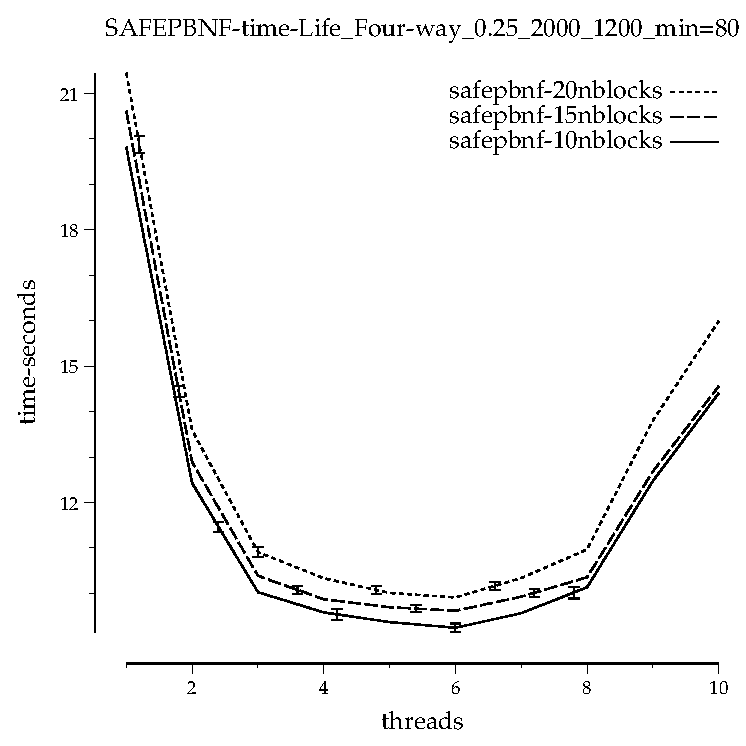
\includegraphics[width=3in]{../graphs/grid_life_four-way_0.25_2000_1200/SAFEPBNF-time-Life_Four-way_0.25_2000_1200_min=80.eps}
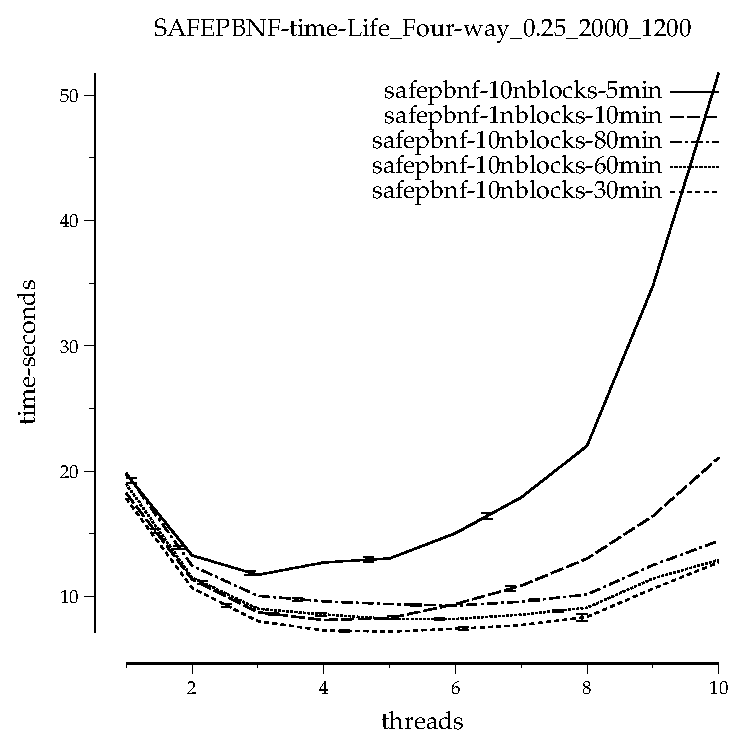
\includegraphics[width=3in]{../graphs/grid_life_four-way_0.25_2000_1200/SAFEPBNF-time-Life_Four-way_0.25_2000_1200.eps}
\caption{Safe PBNF on life cost grid world boards.}
\label{fig:SafePBNF-life}
\end{figure*}

\begin{figure}[h!]
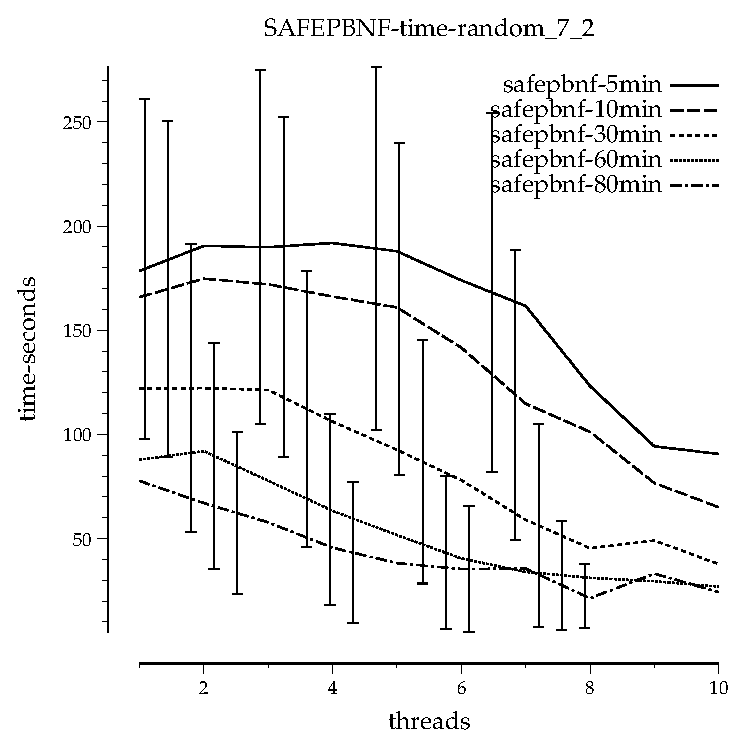
\includegraphics[width=3in]{../graphs/tiles_random_7_2/SAFEPBNF-time-random_7_2.eps}
\caption{Different values for minimum expansions in Safe PBNF on 7x2 sliding tile puzzles.}
\label{fig:SafePBNF-tile}
\end{figure}
\end{appendices}

\end{document}
